\subsection{Rating System Analysis}
\label{sec:rating-analysis}

Most LLM evaluation arenas use Bradley--Terry models (batch MLE) without reporting uncertainty---a potentially misleading practice. We stress-tested four ranking systems (Bradley--Terry, Elo, Glicko-1, and GXE) across 1.6M+ agent matches (Figure~\ref{fig:rating_systems}). Top-3 agents converged across all methods (with 250+ games each), but ranks 4+ showed systematic disagreement---Elo diverged from Bradley--Terry even when error bars did not overlap. Glicko-1 offered the best tradeoff: online updates for real-time leaderboards with convergence guarantees matching batch MLE. We prefer Glicko-1 over raw Elo for agent evaluation, particularly when sample sizes vary across agents. Figure \ref{fig:track1_qualifying_scatter_appendix} compares the Battling Track competition results according to alternative skill metrics (Showdown's Elo, GXE, Win Rate) and sample size (Battles Played).

\begin{figure}[h]
    \centering
    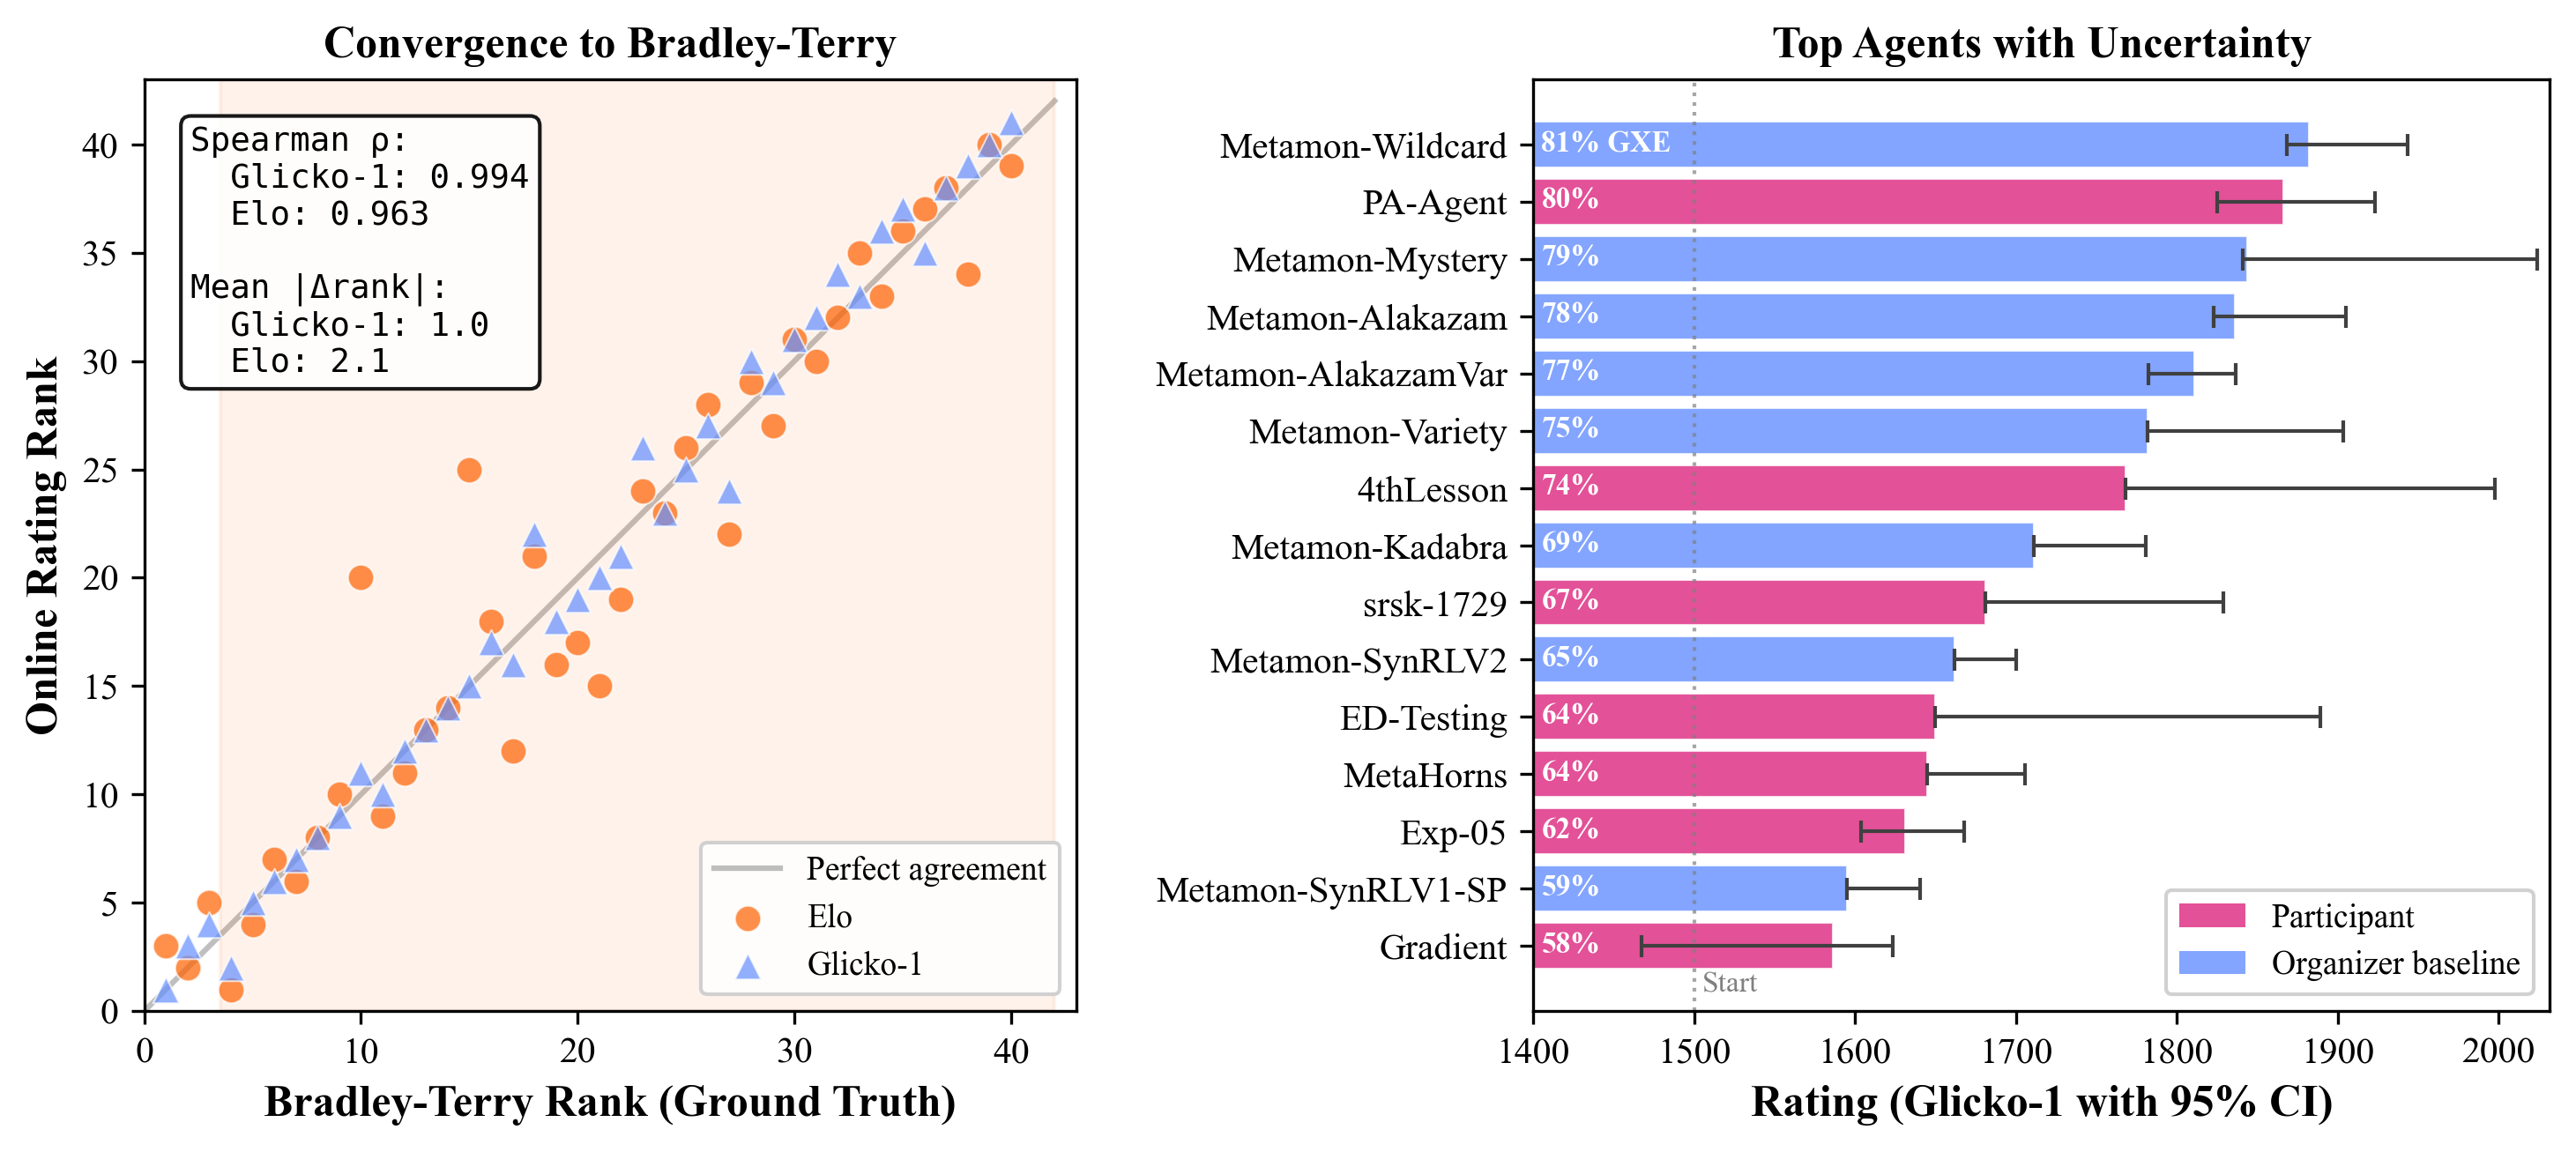
\includegraphics[width=0.95\linewidth]{figures/rating_systems.png}
    \caption{\textbf{Rating System Comparison Across 1.6M+ Matches.} Four ranking methods applied to Battling Track data. Left: Rank correlation between methods, showing Glicko-1 converges to Bradley--Terry (batch MLE) while Elo diverges for mid-ranked agents. Right: Rating trajectories with uncertainty bands for selected agents, demonstrating Glicko-1's uncertainty quantification. Top-3 agents (shaded) show consistent rankings across methods; ranks 4+ exhibit systematic disagreement, particularly between Elo and Bradley--Terry.
    }
    \label{fig:rating_systems}
\end{figure}


\begin{figure}
    \centering
    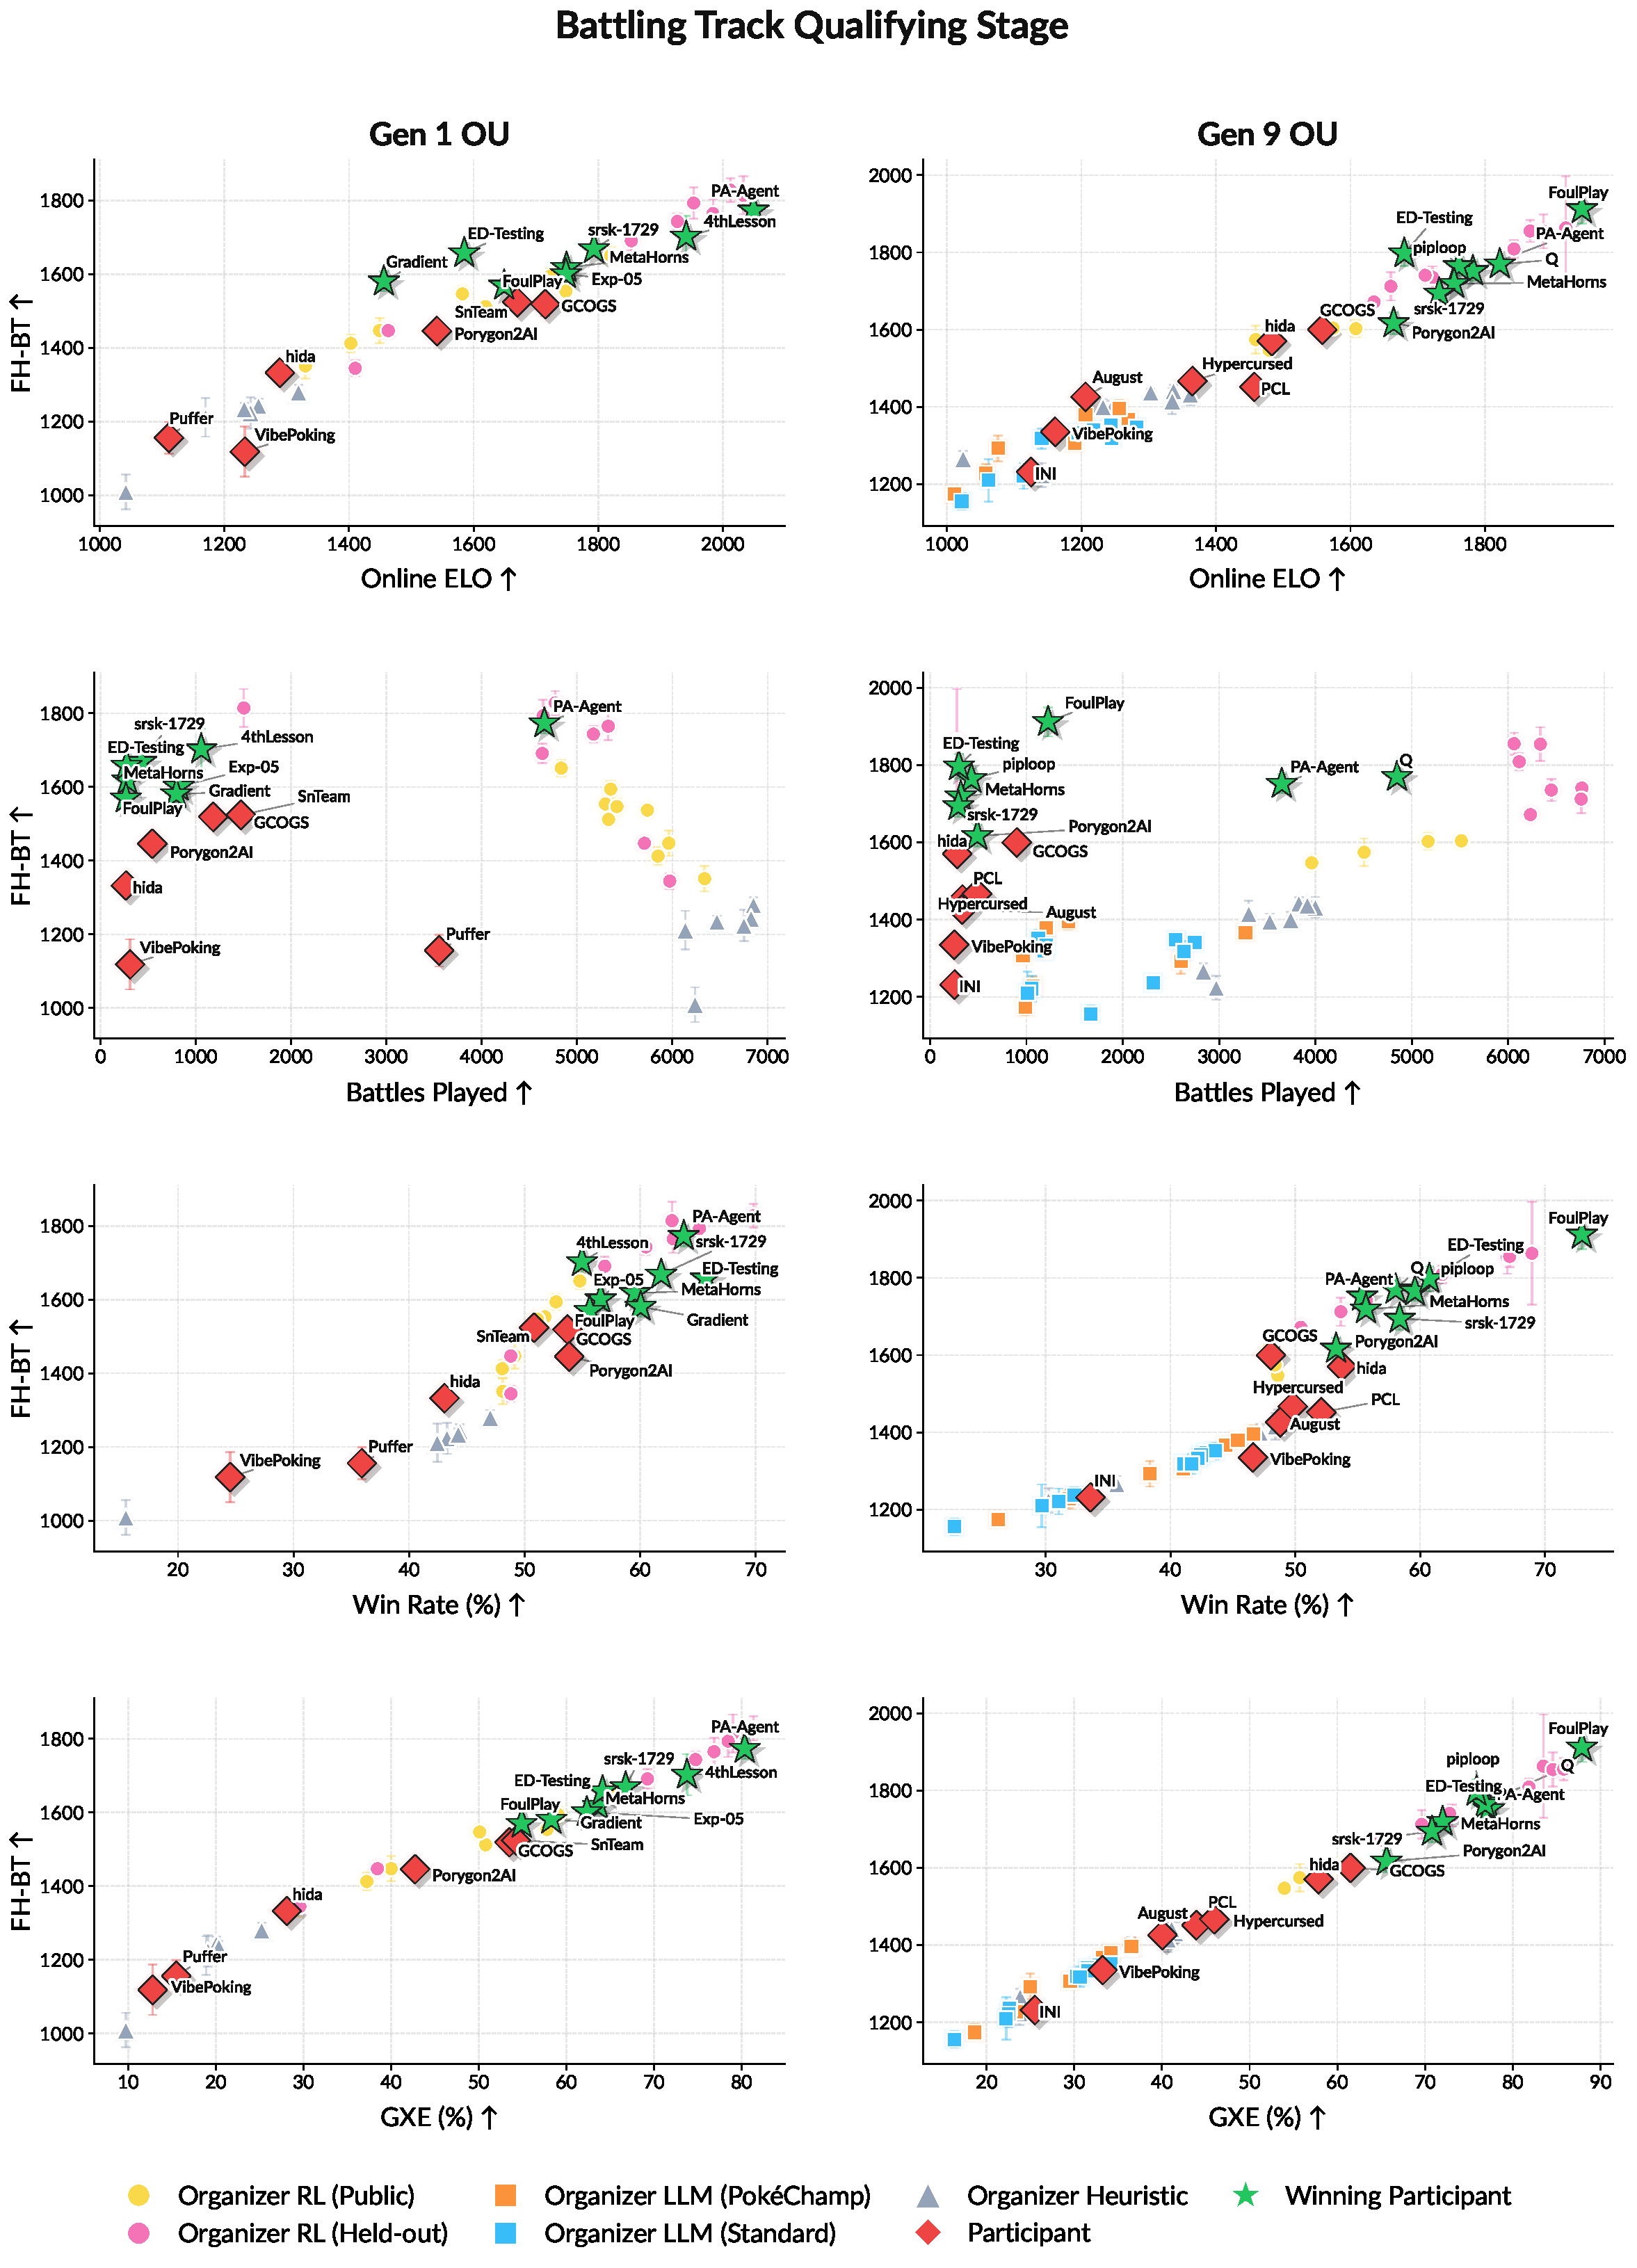
\includegraphics[width=\linewidth]{figures/track1_qualifying_scatter_appendix.pdf}
    \vspace{2mm}
    \caption{\textbf{Battling Track Qualifying Metrics.} Qualifying stage results according to alternative skill metrics (Showdown's Elo, GXE, Win Rate) and sample size (Battles Played). }
    \label{fig:track1_qualifying_scatter_appendix}
\end{figure}
